\documentclass[compress, aspectratio=169]{beamer}
\usepackage[utf8]{inputenc}
\usepackage{braket}
\newcommand{\identity}[0]{\mathbf{1}}
\newcommand{\Op}[1]{\ensuremath{\mathsf{\hat{#1}}}}
\newcommand{\TildeOp}[1]{\ensuremath{\mathsf{\tilde{#1}}}}
\newcommand{\Abs}[1]{\left|#1\right|}
\newcommand{\AbsSq}[1]{\left|#1\right|^2}
\newcommand{\Norm}[1]{\left\lVert#1\right\rVert}
\newcommand{\NormSq}[1]{\Norm{#1}^2}
\newcommand{\tr}{\mathsf{tr}}
\newcommand{\Tr}{\mathsf{tr}}
\newcommand{\SU}{\ensuremath{\text{SU}}}
\newcommand{\ketbra}[2]{\ket{#1}\!\bra{#2}}
\newcommand{\mirror}{\text{mirror}}
\newcommand{\tgt}{\text{tgt}}
\newcommand{\pop}{\operatorname{pop}}
\newcommand{\dd}{\mathsf{d}}
\newcommand{\ii}{\mathsf{i}}
\newcommand{\Integers}{\mathbb{Z}}
\renewcommand{\Re}{\mathsf{Re}}
\renewcommand{\Im}{\mathsf{Im}}
\newcommand{\partdifquo}[2][{}]{\frac{\partial #1}{\partial #2}}
\newcommand{\Complex}{\mathbb{C}}
\usepackage{textcomp} % provides \textmu
\usepackage{tikz,pgflibraryshapes}
\usepackage{hyperref}
\usepackage{fontawesome}
\usetikzlibrary{arrows.meta, calc, decorations.pathmorphing, backgrounds, positioning}

%% Notes on screenshots:
%
% - Make sure ``Reduce Transparency'' in the Accessibility settings (Display) is off
% - Size window to 1270 x 625
% - Take screenshots at retina resolution
% - Terminal (iTerm) is at standard size +5 font size increases


%%%%%%%%%%%%%%%%%%%%%%%%%%%%%%%%%%%%%%%%%%%%%%%%%%%%%%%%%%%%%%%%%%%%%%%%%%%%%%%%
% This theme is for ARL slides in widescreen (16:9) format
%
% Usage: use beamer class
%
%     \documentclass[12pt, compress, aspectratio=169]{beamer}
%
% and e.g.
%
%     %%%%%%%%%%%%%%%%%%%%%%%%%%%%%%%%%%%%%%%%%%%%%%%%%%%%%%%%%%%%%%%%%%%%%%%%%%%%%%%%
% This theme is for ARL slides in widescreen (16:9) format
%
% Usage: use beamer class
%
%     \documentclass[12pt, compress, aspectratio=169]{beamer}
%
% and e.g.
%
%     %%%%%%%%%%%%%%%%%%%%%%%%%%%%%%%%%%%%%%%%%%%%%%%%%%%%%%%%%%%%%%%%%%%%%%%%%%%%%%%%
% This theme is for ARL slides in widescreen (16:9) format
%
% Usage: use beamer class
%
%     \documentclass[12pt, compress, aspectratio=169]{beamer}
%
% and e.g.
%
%     \input{arlwide_theme/theme.tex}
%     \title[Optimal pulse schemes for atom interferometry]{%
%       Optimal pulse schemes \\for high-precision atom interferometry}
%     \author[Michael Goerz (goerz@stanford.edu)]{%
%       {\bf M. Goerz}$^1$, P. Kunz$^1$, M. Kasevich$^2$, V. Malinovsky$^1$
%     }
%     \institute[\protect{\includegraphics[height=5pt]{images/arl}}]{%
%       $^1$U.S. Army Research Lab, $^2$Stanford University
%     }
%     \date{August 23, 2018}
%
% in the header of the tex file. Make sure to disable any footer on the
% titlepage:
%
%     {%  Title page
%       \setbeamertemplate{footline}{}
%       \frame{\titlepage}
%     }
%     \addtocounter{framenumber}{-1}
%
% NOTE: for documentation of how to modify templates, in addition to the Beamer
% user guide, use
% http://www.cpt.univ-mrs.fr/~masson/latex/Beamer-appearance-cheat-sheet.pdf
%
%%%%%%%%%%%%%%%%%%%%%%%%%%%%%%%%%%%%%%%%%%%%%%%%%%%%%%%%%%%%%%%%%%%%%%%%%%%%%%%%
\usepackage{tikz}
\usetikzlibrary{calc}
\usetikzlibrary{positioning}


%%%%%%%%%%%%%%%%%%%%%%%%%%%%%% Grid %%%%%%%%%%%%%%%%%%%%%%%%%%%%%%%%%%%%%%%%%%%%
% Set up grid for absolute text positioning (page size = 16 x 9 cm)
\usepackage[absolute, overlay]{textpos} % (add `showboxes` for debugging)
%\usepackage[absolute, overlay, showboxes]{textpos} % (add `showboxes` for debugging)
\textblockorigin{0cm}{0cm} % The grid guides start from top left
\setlength{\TPHorizModule}{1cm} % Units are 1 cm ...
\setlength{\TPVertModule}{1cm} % ... and y coordinates point down
% Now you can use e.g.:
%    \begin{textblock}{3}(4,2)
%      \dots
%    \end{textblock}
% to place a block 3cm wide, 4cm right and 2cm up from the bottom left corner
%%%%%%%%%%%%%%%%%%%%%%%%%%% Theme Settings %%%%%%%%%%%%%%%%%%%%%%%%%%%%%%%%%%%%%

\definecolor{DarkBlue}{rgb}{0.1,0.1,0.5}
\definecolor{DarkRed}{rgb}{0.75,0.,0.}
\definecolor{Magenta}{rgb}{1.0,0.0,1.0}
\definecolor{Red}{rgb}{0.894,0.102,0.110}
\definecolor{Green}{rgb}{0.302,0.686,0.290}
\definecolor{Blue}{rgb}{0.216,0.494,0.722}
\definecolor{Orange}{rgb}{1.000,0.498,0.000}
\definecolor{Yellow}{rgb}{0.824,0.824,0.082}
\definecolor{Brown}{rgb}{0.651,0.337,0.157}
\definecolor{LightBlue}{rgb}{0.651,0.808,0.890}
\definecolor{Purple}{rgb}{0.596,0.306,0.639}
\definecolor{LightPurple}{rgb}{0.792,0.698,0.839}
\definecolor{Grey}{rgb}{0.600,0.600,0.600}
\definecolor{LightGreen}{rgb}{0.698,0.875,0.541}
\definecolor{LightOrange}{rgb}{0.992,0.749,0.435}
\definecolor{Pink}{rgb}{0.969,0.506,0.749}
\definecolor{Black}{rgb}{0.000,0.000,0.000}
\definecolor{LightRed}{rgb}{0.984,0.604,0.600}
\definecolor{White}{rgb}{1.000,1.000,1.000}

\definecolor{ARLGray25}{rgb}{0.698,0.698,0.698}


%%%%%%%%%%%%%%%%%%%%%%%%%%% Theme Settings %%%%%%%%%%%%%%%%%%%%%%%%%%%%%%%%%%%%%
\usetheme{Berlin}
\useoutertheme{shadow}
\useinnertheme{default}
\setbeamercolor{palette primary}{use=structure,fg=black,bg=black!20!white}
\setbeamercolor{palette secondary}{use=structure,fg=black,bg=black!25!white}
\setbeamercolor{palette tertiary}{use=structure,fg=black,bg=black!30!white}
\setbeamercolor{palette quaternary}{use=structure,fg=black,bg=black!35!white}
\setbeamercolor{sidebar}{use=structure,bg=structure.fg!20!white}
\setbeamercolor{palette sidebar primary}{use=normal text,fg=normal text.fg}
\setbeamercolor{palette sidebar secondary}{use=structure,fg=structure.fg}
\setbeamercolor{palette sidebar tertiary}{use=normal text,fg=normal text.fg}
\setbeamercolor{palette sidebar quaternary}{use=structure,fg=structure.fg}
\setbeamercolor*{titlelike}{parent=palette primary}
\setbeamercolor*{separation line}{}
\setbeamercolor*{fine separation line}{}
\setbeamertemplate{blocks}[rounded][shadow=false]
\setbeamerfont{title}{family*=phv, size*={20}{24}}
\setbeamerfont{author}{family*=phv, size*={12}{14}}
\setbeamerfont{institute}{family*=phv, size*={8.0}{12}}
\setbeamerfont{date}{family*=phv, size*={8.0}{12}}
\setbeamerfont{classification}{family*=phv, size*={3.78}{4.5}}
\setbeamerfont{frametitle}{series=\bfseries, family*=phv, size*={11.34}{14}}
\defbeamertemplate*{title page}{customized}[1][]{%
  \tikz[overlay,remember picture] (current page.south west) rectangle (current page.north east);
  \begin{textblock}{14}(0.0,0.0)
    
\includegraphics[width=\textwidth]{arlwide_theme/arl_devcom_title}
  \end{textblock}
  \begin{textblock}{14}(1,2.8)
    \begin{center}
      {\color{black} \usebeamerfont{title} \inserttitle}
    \end{center}
  \end{textblock}
  \begin{textblock}{14}(1,5.0)
    \begin{center}
      {\color{black} \usebeamerfont{author} \insertauthor}
    \end{center}
  \end{textblock}
  \begin{textblock}{14}(1,6.25)
    \begin{center}
      {\color{black} \usebeamerfont{institute} \insertinstitute}
    \end{center}
  \end{textblock}
  \begin{textblock}{14}(1,7.5)
    \begin{center}
      {\color{black} \usebeamerfont{date} \insertdate}
    \end{center}
  \end{textblock}
}
\setbeamertemplate{background canvas}{%
  % textblock does not work in background canvas, for some reason
  %\tikz[overlay,remember picture] \node[at=(current page.center)]{%
    %\includegraphics[height=\paperheight,width=\paperwidth]
    %{arlwide_theme/titleexample.pdf}};
  \begin{tikzpicture}[remember picture, overlay]
    %%% grid for positioning (debugging)
    %\draw[step=1cm, color=blue, opacity=0.2]
    %(current page.south west) grid (current page.north east);
    %\foreach \x in {0,...,15}{%
    %  \node[inner sep = 0, below right = 3mm and \x of current page.north west]
    %  {\tiny\x};}
    %\foreach \y in {1,...,8}{%
    %  \node[inner sep = 0, below right = \y and 0mm of current page.north west]
    %  {\tiny\y};}
    %%%%
    \node[above=-1.5pt] at (current page.south)
      {\color{ARLGray25} \usebeamerfont{classification} UNCLASSIFIED};
    %\node[below=-1.5pt] at (current page.north)
    %  {\color{ARLGray25} \usebeamerfont{classification} UNCLASSIFIED};
  \end{tikzpicture}
}

\setbeamertemplate{headline}{}
\setbeamertemplate{footline}{%
  \hbox{%
  \begin{beamercolorbox}[
      wd=1.0\paperwidth,ht=2.5ex,dp=1.125ex,leftskip=.3cm,
      rightskip=.3cm]{}%
    \usebeamerfont{title in head/foot}%
    {\color{gray} \insertshortauthor \hfill%
    \insertframenumber\,/\,\inserttotalframenumber}%
  \end{beamercolorbox}%
  }%
  \begin{tikzpicture}[remember picture, overlay]
    \node[anchor=north east, xshift=-5pt] at (current page.north east) {%
      {\color{gray} \insertshorttitle}};
  \end{tikzpicture}
}

\setbeamertemplate{frametitle}{%
  \begin{center}{\insertframetitle}\end{center}
}


\usefonttheme[onlysmall]{structurebold}
\setbeamertemplate{bibliography item}{%
  \lower2pt\hbox{\pgfuseimage{beamericonarticle}}\insertbiblabel}
\mode<presentation>{\beamertemplatenavigationsymbolsempty}
%\setbeamercolor{block title}{use=structure,fg=white,bg=red!75!black}
%\setbeamercolor{block body}{use=structure,fg=black,bg=red!20!white}

\newcommand{\subhead}[1]{{\bf \color{DarkBlue} #1}}

\newcommand{\mycircledTerm}[1]{\raisebox{-0.6ex}{\textcircled{\scriptsize #1}}}
\newcommand{\mycircled}[1]{\textcircled{\scriptsize #1}}

%%%%%%%%%%%%%%%%%%%%%%%%%%%%%%%%%%%%%%%%%%%%%%%%%%%%%%%%%%%%%%%%%%%%%%%%%%%%%%%%
% Fix appendix numbering, See
% http://tex.stackexchange.com/questions/2541/beamer-frame-numbering-in-appendix
\newcommand{\backupbegin}{%
   \newcounter{framenumberappendix}
   \setcounter{framenumberappendix}{\value{framenumber}}
}
\newcommand{\backupend}{%
   \addtocounter{framenumberappendix}{-\value{framenumber}}
   \addtocounter{framenumber}{\value{framenumberappendix}}
}
%%%%%%%%%%%%%%%%%%%%%%%%%%%%%%%%%%%%%%%%%%%%%%%%%%%%%%%%%%%%%%%%%%%%%%%%%%%%%%%%


%     \title[Optimal pulse schemes for atom interferometry]{%
%       Optimal pulse schemes \\for high-precision atom interferometry}
%     \author[Michael Goerz (goerz@stanford.edu)]{%
%       {\bf M. Goerz}$^1$, P. Kunz$^1$, M. Kasevich$^2$, V. Malinovsky$^1$
%     }
%     \institute[\protect{\includegraphics[height=5pt]{images/arl}}]{%
%       $^1$U.S. Army Research Lab, $^2$Stanford University
%     }
%     \date{August 23, 2018}
%
% in the header of the tex file. Make sure to disable any footer on the
% titlepage:
%
%     {%  Title page
%       \setbeamertemplate{footline}{}
%       \frame{\titlepage}
%     }
%     \addtocounter{framenumber}{-1}
%
% NOTE: for documentation of how to modify templates, in addition to the Beamer
% user guide, use
% http://www.cpt.univ-mrs.fr/~masson/latex/Beamer-appearance-cheat-sheet.pdf
%
%%%%%%%%%%%%%%%%%%%%%%%%%%%%%%%%%%%%%%%%%%%%%%%%%%%%%%%%%%%%%%%%%%%%%%%%%%%%%%%%
\usepackage{tikz}
\usetikzlibrary{calc}
\usetikzlibrary{positioning}


%%%%%%%%%%%%%%%%%%%%%%%%%%%%%% Grid %%%%%%%%%%%%%%%%%%%%%%%%%%%%%%%%%%%%%%%%%%%%
% Set up grid for absolute text positioning (page size = 16 x 9 cm)
\usepackage[absolute, overlay]{textpos} % (add `showboxes` for debugging)
%\usepackage[absolute, overlay, showboxes]{textpos} % (add `showboxes` for debugging)
\textblockorigin{0cm}{0cm} % The grid guides start from top left
\setlength{\TPHorizModule}{1cm} % Units are 1 cm ...
\setlength{\TPVertModule}{1cm} % ... and y coordinates point down
% Now you can use e.g.:
%    \begin{textblock}{3}(4,2)
%      \dots
%    \end{textblock}
% to place a block 3cm wide, 4cm right and 2cm up from the bottom left corner
%%%%%%%%%%%%%%%%%%%%%%%%%%% Theme Settings %%%%%%%%%%%%%%%%%%%%%%%%%%%%%%%%%%%%%

\definecolor{DarkBlue}{rgb}{0.1,0.1,0.5}
\definecolor{DarkRed}{rgb}{0.75,0.,0.}
\definecolor{Magenta}{rgb}{1.0,0.0,1.0}
\definecolor{Red}{rgb}{0.894,0.102,0.110}
\definecolor{Green}{rgb}{0.302,0.686,0.290}
\definecolor{Blue}{rgb}{0.216,0.494,0.722}
\definecolor{Orange}{rgb}{1.000,0.498,0.000}
\definecolor{Yellow}{rgb}{0.824,0.824,0.082}
\definecolor{Brown}{rgb}{0.651,0.337,0.157}
\definecolor{LightBlue}{rgb}{0.651,0.808,0.890}
\definecolor{Purple}{rgb}{0.596,0.306,0.639}
\definecolor{LightPurple}{rgb}{0.792,0.698,0.839}
\definecolor{Grey}{rgb}{0.600,0.600,0.600}
\definecolor{LightGreen}{rgb}{0.698,0.875,0.541}
\definecolor{LightOrange}{rgb}{0.992,0.749,0.435}
\definecolor{Pink}{rgb}{0.969,0.506,0.749}
\definecolor{Black}{rgb}{0.000,0.000,0.000}
\definecolor{LightRed}{rgb}{0.984,0.604,0.600}
\definecolor{White}{rgb}{1.000,1.000,1.000}

\definecolor{ARLGray25}{rgb}{0.698,0.698,0.698}


%%%%%%%%%%%%%%%%%%%%%%%%%%% Theme Settings %%%%%%%%%%%%%%%%%%%%%%%%%%%%%%%%%%%%%
\usetheme{Berlin}
\useoutertheme{shadow}
\useinnertheme{default}
\setbeamercolor{palette primary}{use=structure,fg=black,bg=black!20!white}
\setbeamercolor{palette secondary}{use=structure,fg=black,bg=black!25!white}
\setbeamercolor{palette tertiary}{use=structure,fg=black,bg=black!30!white}
\setbeamercolor{palette quaternary}{use=structure,fg=black,bg=black!35!white}
\setbeamercolor{sidebar}{use=structure,bg=structure.fg!20!white}
\setbeamercolor{palette sidebar primary}{use=normal text,fg=normal text.fg}
\setbeamercolor{palette sidebar secondary}{use=structure,fg=structure.fg}
\setbeamercolor{palette sidebar tertiary}{use=normal text,fg=normal text.fg}
\setbeamercolor{palette sidebar quaternary}{use=structure,fg=structure.fg}
\setbeamercolor*{titlelike}{parent=palette primary}
\setbeamercolor*{separation line}{}
\setbeamercolor*{fine separation line}{}
\setbeamertemplate{blocks}[rounded][shadow=false]
\setbeamerfont{title}{family*=phv, size*={20}{24}}
\setbeamerfont{author}{family*=phv, size*={12}{14}}
\setbeamerfont{institute}{family*=phv, size*={8.0}{12}}
\setbeamerfont{date}{family*=phv, size*={8.0}{12}}
\setbeamerfont{classification}{family*=phv, size*={3.78}{4.5}}
\setbeamerfont{frametitle}{series=\bfseries, family*=phv, size*={11.34}{14}}
\defbeamertemplate*{title page}{customized}[1][]{%
  \tikz[overlay,remember picture] (current page.south west) rectangle (current page.north east);
  \begin{textblock}{14}(0.0,0.0)
    
\includegraphics[width=\textwidth]{arlwide_theme/arl_devcom_title}
  \end{textblock}
  \begin{textblock}{14}(1,2.8)
    \begin{center}
      {\color{black} \usebeamerfont{title} \inserttitle}
    \end{center}
  \end{textblock}
  \begin{textblock}{14}(1,5.0)
    \begin{center}
      {\color{black} \usebeamerfont{author} \insertauthor}
    \end{center}
  \end{textblock}
  \begin{textblock}{14}(1,6.25)
    \begin{center}
      {\color{black} \usebeamerfont{institute} \insertinstitute}
    \end{center}
  \end{textblock}
  \begin{textblock}{14}(1,7.5)
    \begin{center}
      {\color{black} \usebeamerfont{date} \insertdate}
    \end{center}
  \end{textblock}
}
\setbeamertemplate{background canvas}{%
  % textblock does not work in background canvas, for some reason
  %\tikz[overlay,remember picture] \node[at=(current page.center)]{%
    %\includegraphics[height=\paperheight,width=\paperwidth]
    %{arlwide_theme/titleexample.pdf}};
  \begin{tikzpicture}[remember picture, overlay]
    %%% grid for positioning (debugging)
    %\draw[step=1cm, color=blue, opacity=0.2]
    %(current page.south west) grid (current page.north east);
    %\foreach \x in {0,...,15}{%
    %  \node[inner sep = 0, below right = 3mm and \x of current page.north west]
    %  {\tiny\x};}
    %\foreach \y in {1,...,8}{%
    %  \node[inner sep = 0, below right = \y and 0mm of current page.north west]
    %  {\tiny\y};}
    %%%%
    \node[above=-1.5pt] at (current page.south)
      {\color{ARLGray25} \usebeamerfont{classification} UNCLASSIFIED};
    %\node[below=-1.5pt] at (current page.north)
    %  {\color{ARLGray25} \usebeamerfont{classification} UNCLASSIFIED};
  \end{tikzpicture}
}

\setbeamertemplate{headline}{}
\setbeamertemplate{footline}{%
  \hbox{%
  \begin{beamercolorbox}[
      wd=1.0\paperwidth,ht=2.5ex,dp=1.125ex,leftskip=.3cm,
      rightskip=.3cm]{}%
    \usebeamerfont{title in head/foot}%
    {\color{gray} \insertshortauthor \hfill%
    \insertframenumber\,/\,\inserttotalframenumber}%
  \end{beamercolorbox}%
  }%
  \begin{tikzpicture}[remember picture, overlay]
    \node[anchor=north east, xshift=-5pt] at (current page.north east) {%
      {\color{gray} \insertshorttitle}};
  \end{tikzpicture}
}

\setbeamertemplate{frametitle}{%
  \begin{center}{\insertframetitle}\end{center}
}


\usefonttheme[onlysmall]{structurebold}
\setbeamertemplate{bibliography item}{%
  \lower2pt\hbox{\pgfuseimage{beamericonarticle}}\insertbiblabel}
\mode<presentation>{\beamertemplatenavigationsymbolsempty}
%\setbeamercolor{block title}{use=structure,fg=white,bg=red!75!black}
%\setbeamercolor{block body}{use=structure,fg=black,bg=red!20!white}

\newcommand{\subhead}[1]{{\bf \color{DarkBlue} #1}}

\newcommand{\mycircledTerm}[1]{\raisebox{-0.6ex}{\textcircled{\scriptsize #1}}}
\newcommand{\mycircled}[1]{\textcircled{\scriptsize #1}}

%%%%%%%%%%%%%%%%%%%%%%%%%%%%%%%%%%%%%%%%%%%%%%%%%%%%%%%%%%%%%%%%%%%%%%%%%%%%%%%%
% Fix appendix numbering, See
% http://tex.stackexchange.com/questions/2541/beamer-frame-numbering-in-appendix
\newcommand{\backupbegin}{%
   \newcounter{framenumberappendix}
   \setcounter{framenumberappendix}{\value{framenumber}}
}
\newcommand{\backupend}{%
   \addtocounter{framenumberappendix}{-\value{framenumber}}
   \addtocounter{framenumber}{\value{framenumberappendix}}
}
%%%%%%%%%%%%%%%%%%%%%%%%%%%%%%%%%%%%%%%%%%%%%%%%%%%%%%%%%%%%%%%%%%%%%%%%%%%%%%%%


%     \title[Optimal pulse schemes for atom interferometry]{%
%       Optimal pulse schemes \\for high-precision atom interferometry}
%     \author[Michael Goerz (goerz@stanford.edu)]{%
%       {\bf M. Goerz}$^1$, P. Kunz$^1$, M. Kasevich$^2$, V. Malinovsky$^1$
%     }
%     \institute[\protect{\includegraphics[height=5pt]{images/arl}}]{%
%       $^1$U.S. Army Research Lab, $^2$Stanford University
%     }
%     \date{August 23, 2018}
%
% in the header of the tex file. Make sure to disable any footer on the
% titlepage:
%
%     {%  Title page
%       \setbeamertemplate{footline}{}
%       \frame{\titlepage}
%     }
%     \addtocounter{framenumber}{-1}
%
% NOTE: for documentation of how to modify templates, in addition to the Beamer
% user guide, use
% http://www.cpt.univ-mrs.fr/~masson/latex/Beamer-appearance-cheat-sheet.pdf
%
%%%%%%%%%%%%%%%%%%%%%%%%%%%%%%%%%%%%%%%%%%%%%%%%%%%%%%%%%%%%%%%%%%%%%%%%%%%%%%%%
\usepackage{tikz}
\usetikzlibrary{calc}
\usetikzlibrary{positioning}


%%%%%%%%%%%%%%%%%%%%%%%%%%%%%% Grid %%%%%%%%%%%%%%%%%%%%%%%%%%%%%%%%%%%%%%%%%%%%
% Set up grid for absolute text positioning (page size = 16 x 9 cm)
\usepackage[absolute, overlay]{textpos} % (add `showboxes` for debugging)
%\usepackage[absolute, overlay, showboxes]{textpos} % (add `showboxes` for debugging)
\textblockorigin{0cm}{0cm} % The grid guides start from top left
\setlength{\TPHorizModule}{1cm} % Units are 1 cm ...
\setlength{\TPVertModule}{1cm} % ... and y coordinates point down
% Now you can use e.g.:
%    \begin{textblock}{3}(4,2)
%      \dots
%    \end{textblock}
% to place a block 3cm wide, 4cm right and 2cm up from the bottom left corner
%%%%%%%%%%%%%%%%%%%%%%%%%%% Theme Settings %%%%%%%%%%%%%%%%%%%%%%%%%%%%%%%%%%%%%

\definecolor{DarkBlue}{rgb}{0.1,0.1,0.5}
\definecolor{DarkRed}{rgb}{0.75,0.,0.}
\definecolor{Magenta}{rgb}{1.0,0.0,1.0}
\definecolor{Red}{rgb}{0.894,0.102,0.110}
\definecolor{Green}{rgb}{0.302,0.686,0.290}
\definecolor{Blue}{rgb}{0.216,0.494,0.722}
\definecolor{Orange}{rgb}{1.000,0.498,0.000}
\definecolor{Yellow}{rgb}{0.824,0.824,0.082}
\definecolor{Brown}{rgb}{0.651,0.337,0.157}
\definecolor{LightBlue}{rgb}{0.651,0.808,0.890}
\definecolor{Purple}{rgb}{0.596,0.306,0.639}
\definecolor{LightPurple}{rgb}{0.792,0.698,0.839}
\definecolor{Grey}{rgb}{0.600,0.600,0.600}
\definecolor{LightGreen}{rgb}{0.698,0.875,0.541}
\definecolor{LightOrange}{rgb}{0.992,0.749,0.435}
\definecolor{Pink}{rgb}{0.969,0.506,0.749}
\definecolor{Black}{rgb}{0.000,0.000,0.000}
\definecolor{LightRed}{rgb}{0.984,0.604,0.600}
\definecolor{White}{rgb}{1.000,1.000,1.000}

\definecolor{ARLGray25}{rgb}{0.698,0.698,0.698}


%%%%%%%%%%%%%%%%%%%%%%%%%%% Theme Settings %%%%%%%%%%%%%%%%%%%%%%%%%%%%%%%%%%%%%
\usetheme{Berlin}
\useoutertheme{shadow}
\useinnertheme{default}
\setbeamercolor{palette primary}{use=structure,fg=black,bg=black!20!white}
\setbeamercolor{palette secondary}{use=structure,fg=black,bg=black!25!white}
\setbeamercolor{palette tertiary}{use=structure,fg=black,bg=black!30!white}
\setbeamercolor{palette quaternary}{use=structure,fg=black,bg=black!35!white}
\setbeamercolor{sidebar}{use=structure,bg=structure.fg!20!white}
\setbeamercolor{palette sidebar primary}{use=normal text,fg=normal text.fg}
\setbeamercolor{palette sidebar secondary}{use=structure,fg=structure.fg}
\setbeamercolor{palette sidebar tertiary}{use=normal text,fg=normal text.fg}
\setbeamercolor{palette sidebar quaternary}{use=structure,fg=structure.fg}
\setbeamercolor*{titlelike}{parent=palette primary}
\setbeamercolor*{separation line}{}
\setbeamercolor*{fine separation line}{}
\setbeamertemplate{blocks}[rounded][shadow=false]
\setbeamerfont{title}{family*=phv, size*={20}{24}}
\setbeamerfont{author}{family*=phv, size*={12}{14}}
\setbeamerfont{institute}{family*=phv, size*={8.0}{12}}
\setbeamerfont{date}{family*=phv, size*={8.0}{12}}
\setbeamerfont{classification}{family*=phv, size*={3.78}{4.5}}
\setbeamerfont{frametitle}{series=\bfseries, family*=phv, size*={11.34}{14}}
\defbeamertemplate*{title page}{customized}[1][]{%
  \tikz[overlay,remember picture] (current page.south west) rectangle (current page.north east);
  \begin{textblock}{14}(0.0,0.0)
    
\includegraphics[width=\textwidth]{arlwide_theme/arl_devcom_title}
  \end{textblock}
  \begin{textblock}{14}(1,2.8)
    \begin{center}
      {\color{black} \usebeamerfont{title} \inserttitle}
    \end{center}
  \end{textblock}
  \begin{textblock}{14}(1,5.0)
    \begin{center}
      {\color{black} \usebeamerfont{author} \insertauthor}
    \end{center}
  \end{textblock}
  \begin{textblock}{14}(1,6.25)
    \begin{center}
      {\color{black} \usebeamerfont{institute} \insertinstitute}
    \end{center}
  \end{textblock}
  \begin{textblock}{14}(1,7.5)
    \begin{center}
      {\color{black} \usebeamerfont{date} \insertdate}
    \end{center}
  \end{textblock}
}
\setbeamertemplate{background canvas}{%
  % textblock does not work in background canvas, for some reason
  %\tikz[overlay,remember picture] \node[at=(current page.center)]{%
    %\includegraphics[height=\paperheight,width=\paperwidth]
    %{arlwide_theme/titleexample.pdf}};
  \begin{tikzpicture}[remember picture, overlay]
    %%% grid for positioning (debugging)
    %\draw[step=1cm, color=blue, opacity=0.2]
    %(current page.south west) grid (current page.north east);
    %\foreach \x in {0,...,15}{%
    %  \node[inner sep = 0, below right = 3mm and \x of current page.north west]
    %  {\tiny\x};}
    %\foreach \y in {1,...,8}{%
    %  \node[inner sep = 0, below right = \y and 0mm of current page.north west]
    %  {\tiny\y};}
    %%%%
    \node[above=-1.5pt] at (current page.south)
      {\color{ARLGray25} \usebeamerfont{classification} UNCLASSIFIED};
    %\node[below=-1.5pt] at (current page.north)
    %  {\color{ARLGray25} \usebeamerfont{classification} UNCLASSIFIED};
  \end{tikzpicture}
}

\setbeamertemplate{headline}{}
\setbeamertemplate{footline}{%
  \hbox{%
  \begin{beamercolorbox}[
      wd=1.0\paperwidth,ht=2.5ex,dp=1.125ex,leftskip=.3cm,
      rightskip=.3cm]{}%
    \usebeamerfont{title in head/foot}%
    {\color{gray} \insertshortauthor \hfill%
    \insertframenumber\,/\,\inserttotalframenumber}%
  \end{beamercolorbox}%
  }%
  \begin{tikzpicture}[remember picture, overlay]
    \node[anchor=north east, xshift=-5pt] at (current page.north east) {%
      {\color{gray} \insertshorttitle}};
  \end{tikzpicture}
}

\setbeamertemplate{frametitle}{%
  \begin{center}{\insertframetitle}\end{center}
}


\usefonttheme[onlysmall]{structurebold}
\setbeamertemplate{bibliography item}{%
  \lower2pt\hbox{\pgfuseimage{beamericonarticle}}\insertbiblabel}
\mode<presentation>{\beamertemplatenavigationsymbolsempty}
%\setbeamercolor{block title}{use=structure,fg=white,bg=red!75!black}
%\setbeamercolor{block body}{use=structure,fg=black,bg=red!20!white}

\newcommand{\subhead}[1]{{\bf \color{DarkBlue} #1}}

\newcommand{\mycircledTerm}[1]{\raisebox{-0.6ex}{\textcircled{\scriptsize #1}}}
\newcommand{\mycircled}[1]{\textcircled{\scriptsize #1}}

%%%%%%%%%%%%%%%%%%%%%%%%%%%%%%%%%%%%%%%%%%%%%%%%%%%%%%%%%%%%%%%%%%%%%%%%%%%%%%%%
% Fix appendix numbering, See
% http://tex.stackexchange.com/questions/2541/beamer-frame-numbering-in-appendix
\newcommand{\backupbegin}{%
   \newcounter{framenumberappendix}
   \setcounter{framenumberappendix}{\value{framenumber}}
}
\newcommand{\backupend}{%
   \addtocounter{framenumberappendix}{-\value{framenumber}}
   \addtocounter{framenumber}{\value{framenumberappendix}}
}
%%%%%%%%%%%%%%%%%%%%%%%%%%%%%%%%%%%%%%%%%%%%%%%%%%%%%%%%%%%%%%%%%%%%%%%%%%%%%%%%



\title{Optimal Control of a \\Sagnac Tractor Atom Interferometer}
\author[Michael Goerz~\raisebox{0.75pt}{\tikz \fill (0,0) circle (0.75pt);}~\raisebox{-1.4pt}{
\includegraphics{images/mastodon}}\kern-0.5pt\href{https://qubit-social.xyz/@goerz}{goerz@qubit-social.xyz}]{
  {\bf Michael~H.~Goerz$^1$}, \\{\small B.~Dash$^2$, S.~C.~Carrasco$^1$, A.~Duspayev$^2$, G.~Raithel$^2$, V.~S.~Malinovsky$^1$}}
\institute[Army Research Lab]{$^1$ DEVCOM Army Research Lab, $^2$ Dept. of Physics, U Michigan}
\date{DAMOP Meeting 2023}

\begin{document}

{%  Title page
  \setbeamertemplate{footline}{}
  \frame{\titlepage}
}
\addtocounter{framenumber}{-1}

\begin{frame}{Pinwheel Optical Lattice}
  \begin{textblock}{3.7}(3.0,1.50)
    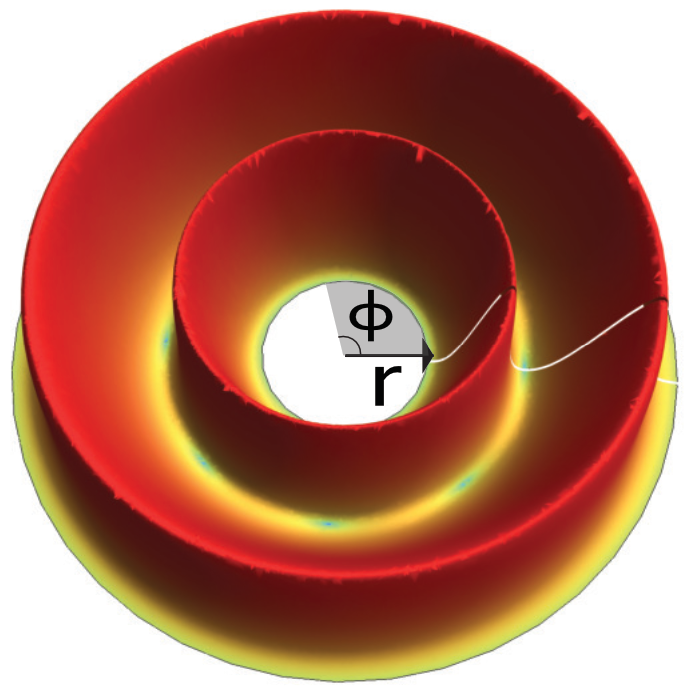
\includegraphics[width=\textwidth]{images/pinwheel.png}
  \end{textblock}
  \begin{textblock}{8.5}(2.5,5.50)
    {\footnotesize
      Franke-Arnold \emph{et al.} Opt. Express 15, 8619 (2007)
    }
  \end{textblock}
  \begin{textblock}{3.7}(8.0,1.50)
    \includegraphics<2->[width=\textwidth]{images/pinwheelzoom.png}
  \end{textblock}
  \begin{textblock}{7}(2.0,7.0)
    \onslide<3>{%
      {\bf\color{DarkRed}Make it spin-dependent!}
      \par
      {\footnotesize
        Raithel \emph{et al.} Quantum Sci. Technol. 8 (2023)
      }
    }
  \end{textblock}
  \begin{textblock}{4.7}(9.25,6.5)
    \onslide<3>{%
      Rubidium-87 hyperfine levels
      \vspace{-8mm}
      \begin{align*}
        \ket{+} &\equiv \ket{F=1, m_F=0} \\
        \ket{-} &\equiv \ket{F=2, m_F=0}
      \end{align*}
    }
  \end{textblock}
\end{frame}


\begin{frame}{Rotating Tractor Interferometer}
  \begin{textblock}{7.0}(0.5,1.70)
    %\includegraphics[width=\textwidth]{images/rottai}
    \includegraphics{images/rottai}\\
    {\footnotesize
      B. Dash \emph{et al.} ``Rotation sensing using tractor atom interferometry'' (in preparation)
    }
  \end{textblock}
  \begin{textblock}{7.5}(8.0,3.00)
    \begin{equation*}
      \Op{H}_{\pm}
        = -\frac{\hbar^2}{2M}\frac{\partial^2}{\partial \theta^2} +
          \underbrace{V_0 \cos\left[m (\theta + {\color<2>{DarkRed}\phi_{\pm}(t)} )\right]}_{=V_{\pm}(\theta, t)}
    \end{equation*}
  \end{textblock}
  \begin{textblock}{7.5}(8.0,4.70)
    \onslide<2->{%
      \begin{equation*}
        \phi_{\pm}(t)
        = \int_{0}^{t} \omega_{\pm}(t^\prime)\,dt^\prime
        = \int_{0}^{t}\left( {\color<3>{DarkRed}\Omega} \pm \omega(t^\prime)\right)\,dt^\prime
      \end{equation*}
    }
  \end{textblock}
\end{frame}


\begin{frame}{Adiabatic Dynamics}
  \begin{textblock}{7.0}(0.5,1.00)
    \includegraphics<1-4>{images/animate_rottai/frame_000.pdf}
    \includegraphics<5>{images/animate_rottai/frame_100.pdf}
    \includegraphics<6>{images/animate_rottai/frame_200.pdf}
    \includegraphics<7->{images/animate_rottai/frame_300.pdf}
  \end{textblock}
  \begin{textblock}{7.0}(0.5,2.00)
    \onslide<2>{%
      \begin{center}
        {\color{DarkRed}$\pi/2$ pulse}
      \end{center}
    }
  \end{textblock}
  \begin{textblock}{7.0}(0.5,2.00)
    \onslide<9>{%
      \begin{center}
        {\color{DarkRed}inverse \\ $\pi/2$ pulse}
      \end{center}
    }
  \end{textblock}
  \begin{textblock}{7.0}(0.5,5.50)
    \onslide<3->{%
      \begin{equation*}
        \omega(t) = \begin{cases}
          \omega_{0} \sin^2\left(\frac{\pi t}{2 t_r}\right)         & 0 \leq t < t_r            \\
          \omega_{0}                                                & t_r \leq t < t_r + t_{\text{loop}}  \\
          \omega_{0} \cos^2\left(\frac{\pi t^\prime }{2t_r} \right) & T - t_r \leq t \leq T
        \end{cases}
      \end{equation*}
    }
  \end{textblock}
  \begin{textblock}{7.5}(8.0,3.00)
    \onslide<1-3>{
      \begin{equation*}
        \Op{H}_{\pm}
          = -\frac{\hbar^2}{2M}\frac{\partial^2}{\partial \theta^2} +
            \underbrace{V_0 \cos\left[m (\theta + {\phi_{\pm}(t)} )\right]}_{=V_{\pm}(\theta, t)}
      \end{equation*}
    }
  \end{textblock}
  \begin{textblock}{7.5}(8.0,4.70)
    \onslide<1-3>{
      \begin{equation*}
        \phi_{\pm}(t)
        = \int_{0}^{t} \omega_{\pm}(t^\prime)\,dt^\prime
        = \int_{0}^{t}\left( {\Omega} \pm \omega(t^\prime)\right)\,dt^\prime
      \end{equation*}
    }
  \end{textblock}
  \begin{textblock}{7.75}(8.0,2.00)
    \begin{center}
      \includegraphics<4-7>{images/adiabatic_dynamics_50πps_1}
      \includegraphics<8->{images/adiabatic_dynamics_50πps_2}
    \end{center}
  \end{textblock}
\end{frame}

\begin{frame}{Interferometric Response}
  \begin{textblock}{15.5}(0.25,1.30)
    \begin{equation*}
      \Delta \Phi_S = \frac{4 m\Omega A}{\hbar}\,,
      \quad
      A
      = \frac{R^2}{2}
        \underbrace{\int_{0}^{T}\omega(t^\prime)dt^\prime}_{=\only<1-4>{n}\only<5>{2}\only<6>{10}\pi}
    \end{equation*}
  \end{textblock}
  \begin{textblock}{15.5}(0.25,3.00)
    \onslide<2->{%
      \begin{equation*}
        |c_{\pm}|^2
        = \frac{1}{2}
          \pm \frac{1}{2} \Re\left[{\color<3>{DarkRed}\eta} e^{-i \Delta\Phi}\right]
        \onslide<4->{%
          \qquad \rightarrow  \qquad
          |c_{-}|^2
          = \frac{1}{2} - \frac{\cos{\Delta\Phi}}{2} = \sin^2\left(\frac{\Delta\Phi}{2}\right)
        }
      \end{equation*}
    }
  \end{textblock}
  \begin{textblock}{4}(1.85,4.00)
    \onslide<3-4>{%
      \begin{equation*}
        \color{DarkRed}
        \eta = \braket{\Psi_{-}(\theta, T)|\Psi_{+}(\theta, T)}
        = 1 \quad \text{if adiabatic}
      \end{equation*}
    }
  \end{textblock}
  \begin{textblock}{15.5}(0.25,4.2)
    \onslide<5->{%
      \begin{center}
        \includegraphics<5>{images/cn_sim_results_1.pdf}
        \includegraphics<6>{images/cn_sim_results_2.pdf}
      \end{center}
    }
  \end{textblock}
\end{frame}


\begin{frame}{Non-Adiabatic Dynamics}
  \begin{textblock}{7.75}(0.25,2.00)
    \includegraphics<1>{images/fidelity_map_1}
    \includegraphics<2-8>{images/fidelity_map_2}
  \end{textblock}
  \begin{textblock}{7.0}(8.5,2.25)
    \onslide<1-2>{%
      \begin{equation*}
        \omega(t) = \begin{cases}
          \omega_{0} \sin^2\left(\frac{\pi t}{2 t_r}\right)         & 0 \leq t < t_r            \\
          {\color{gray}\omega_{0}}                                  & {\color{gray}t_r \leq t < t_r + t_{\text{loop}}}  \\
          {\color{gray}\omega_{0} \cos^2\left(\frac{\pi t^\prime }{2t_r} \right)} & {\color{gray}T - t_r \leq t \leq T}
        \end{cases}
      \end{equation*}
      \vspace{2mm}
      \par
      $\ket{\Psi_{\text{tgt}}} = $ ground state of moving potential
    }
  \end{textblock}
  \begin{textblock}{7.75}(8.00,1.00)
    \includegraphics<3>{images/guess_dynamics_1.pdf}
    \includegraphics<4>{images/guess_dynamics_2.pdf}
    \includegraphics<5>{images/guess_dynamics_3.pdf}
    \includegraphics<6>{images/guess_dynamics_4.pdf}
    \includegraphics<7>{images/guess_dynamics_5.pdf}
    \includegraphics<8->{images/guess_dynamics_6.pdf}
  \end{textblock}
  \begin{textblock}{7.75}(0.25,2.00)
    \includegraphics<9-11>{images/guess_sagnac_1.pdf}
    \includegraphics<12>{images/guess_sagnac_2.pdf}
  \end{textblock}
  \begin{textblock}{7.75}(0.25,5.75)
    \onslide<9->{%
      \begin{equation*}
        \Delta \Phi_S = \frac{4 m\Omega A}{\hbar}\,,
        \quad
        A = \frac{R^2}{2} \cdot 10\pi
      \end{equation*}
    }
  \end{textblock}
  \begin{textblock}{7.75}(0.25,7.00)
    \only<9>{%
      \begin{equation*}
        |c_{-}|^2
        = \frac{1}{2} - \frac{\cos{\Delta\Phi}}{2} = \sin^2\left(\frac{\Delta\Phi}{2}\right)
      \end{equation*}
    }
    \only<10->{%
      \begin{equation*}
        |c_{-}|^2
        = \frac{1}{2} - \frac{1}{2} \Re\left[{\color<11>{DarkRed}\eta} e^{-i \Delta\Phi}\right]
      \end{equation*}
    }
  \end{textblock}
\end{frame}

\begin{frame}{Control Problem}

  \begin{textblock}{15.0}(0.5,1.20)
    \begin{center}
      \begin{equation*}
        \omega(t) = \begin{cases}
          \omega_{\text{opt}}(t)  & 0 \leq t < t_r            \\
          \omega_{0}              & t_r \leq t < t_r + t_{\text{loop}}  \\
          \omega_{\text{opt}}(t') & T - t_r \leq t \leq T
        \end{cases}
      \end{equation*}
      \par
      \vspace{8mm}
      Find $\omega_{\text{opt}}(t)$ for short $t_r$ so that
      \begin{equation*}
        \color{DarkRed}
        \Psi(\theta, t=0) \rightarrow \Psi_{\text{tgt}}(\theta, t=t_r)
      \end{equation*}
      where $\ket{\Psi_{\text{tgt}}} = $ ground state of moving potential
    \end{center}
  \end{textblock}

\end{frame}

\begin{frame}{Optimization with QuantumControl.jl}
  \begin{textblock}{15.5}(0.25,1.00)
    \includegraphics<1-2>[width=\textwidth]{images/juliaquantumcontrol}
    \includegraphics<3-5>[width=\textwidth]{images/optimization_screenshot1}
    \includegraphics<6>[width=\textwidth]{images/optimization_screenshot2}
  \end{textblock}
  \begin{textblock}{14}(1.0,4.55)
    \onslide<2>{%
      \begin{block}{2023 APS March Meeting}
        \vspace{3mm}
        ``QuantumControl.jl: A modern framework for quantum optimal control.''
        \par\vspace{3mm}
        \url{https://www.youtube.com/watch?v=2_6KC89pTJI}
        \vspace{3mm}
      \end{block}
    }
  \end{textblock}
  \begin{textblock}{12.8}(2.0,3.70)
    \onslide<4>{%
      \begin{block}{Guided Control}
        \vspace{2mm}
        \begin{equation*}
          \omega_{\text{opt}}(t) = \omega(t) + S(t)\delta\omega(t)
        \end{equation*}
        \vspace{2mm}
      \end{block}
    }
  \end{textblock}
\end{frame}

\begin{frame}{Optimized Dynamics}
  \begin{textblock}{7.75}(0.25,1.00)
    \includegraphics<1-6>{images/guess_dynamics.pdf}
  \end{textblock}
  \begin{textblock}{7.75}(8.00,1.00)
    \includegraphics<2>{images/opt_dynamics_1.pdf}
    \includegraphics<3>{images/opt_dynamics_2.pdf}
    \includegraphics<4>{images/opt_dynamics_3.pdf}
    \includegraphics<5>{images/opt_dynamics_5.pdf}
    \includegraphics<6->{images/opt_dynamics_6.pdf}
  \end{textblock}
  \begin{textblock}{7.75}(0.25,2.00)
    \includegraphics<7>{images/opt_sagnac_1.pdf}
    \includegraphics<8->{images/opt_sagnac_2.pdf}
  \end{textblock}
  \begin{textblock}{7.75}(0.25,5.75)
    \onslide<7->{%
      \begin{equation*}
        \Delta \Phi_S = \frac{4 m\Omega A}{\hbar}\,,
        \quad
        A = \frac{R^2}{2} \cdot 10\pi
      \end{equation*}
    }
  \end{textblock}
  \begin{textblock}{7.75}(0.25,7.00)
    \only<7>{%
      \begin{equation*}
        |c_{-}|^2
        = \frac{1}{2} - \frac{1}{2} \Re\left[\eta e^{-i \Delta\Phi}\right]
      \end{equation*}
    }
    \only<8->{%
      \begin{equation*}
        |c_{-}|^2
        = \frac{1}{2} - \frac{\cos{\Delta\Phi}}{2} = \sin^2\left(\frac{\Delta\Phi}{2}\right)
      \end{equation*}
    }
  \end{textblock}
\end{frame}



\begin{frame}{Conclusions}
  \begin{textblock}{14.5}(1.25,1.50)
    \subhead{Tractor Atom Interferometer}
    \begin{itemize}
      \item Pinwheel optical lattice with freely tuneable angular velocity
      \item Can be made spin-dependent (Rubidium hyperfine levels)
      \item Continuous confinement guarantees closure of interferometer (if adiabatic)
      \item Highly scalable due to multi-pass design
    \end{itemize}
    \par
    \vspace{14pt}
    \subhead{Optimal Control}
    \begin{itemize}
      \item Control problem: non-adiabatically go to moving-lattice ground state
      \item Optimization with QuantumControl.jl\\
            \url{https://github.com/JuliaQuantumControl}
      \item ``Throw and catch'' solution restores full contrast
    \end{itemize}
  \end{textblock}
  \begin{textblock}{14}(1,7.89)
    \onslide<2>{%
      \begin{center}
        \textbf{Thank You}
      \end{center}
    }
  \end{textblock}
\end{frame}


\end{document}
